% make sure to compile this with lualatex or it will not work
\documentclass[10pt]{article}
% custom borders for my page
\usepackage[a4paper,top=2cm,bottom=2cm,left=2cm,right=2cm]{geometry}
\usepackage{iftex}
\ifLuaTeX
% use system fonts in latex
\usepackage{fontspec}
% funky font
\newfontface\mollefont[ Scale = 1 ]{Molle-Regular.otf}
\fi
% no headers
\usepackage{rotating}
\usepackage{color}
% graphing fun with pgf/tikz
\usepackage{tikz}
\pagestyle{empty}

\begin{document}
\pagecolor[rgb]{0.8,0.9,0.9}
\vspace*{\stretch{1}}
\begin{center}
\rotatebox{30}{\ifLuaTeX\mollefont\fi\fontsize{2cm}{1.2ex}\selectfont Hello World}
\end{center}
\vspace*{\stretch{1}}
\setlength{\unitlength}{1mm}
\noindent\begin{picture}(0,0)
\put(50,100){\rotatebox{-30}{\parbox[t]{5cm}{
\color[rgb]{1,0.2,0.3}
Lorem ipsum dolor sit amet, consectetur adipiscing elit. Suspendisse sit amet eros ut justo tristique tincidunt mollis eu ligula. Nulla iaculis, nulla vel dictum faucibus, diam magna consequat neque, et auctor eros sem porta felis. In ut sem id nisi scelerisque bibendum. Cum sociis natoque penatibus et magnis dis parturient montes, nascetur ridiculus mus. Nullam aliquam sapien nec risus pulvinar bibendum. Nulla imperdiet cursus vulputate. Morbi eget iaculis nulla. Vestibulum ultricies lectus at leo elementum et gravida quam euismod.
}}}
\end{picture}
\newpage
% http://research.sourcebyte.com/blog/introduction-to-pgftikz/
\begin{tikzpicture}
\draw (0cm,0cm) % coordinate
   -- (5cm,5cm) % coordinate with unit
   -- ++(310:80mm) % relative and move point angle:distance
   -- (380:80mm |- 0cm,0cm) % intersection vertical and horizontal lines
   -- cycle;  % close figure
\end{tikzpicture}

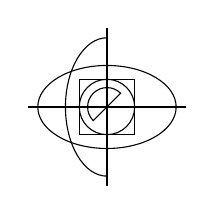
\begin{tikzpicture}
\draw (-1, 0) -- (1, 0);  % x-axis
\draw (0, -1) -- (0, 1);  % y-axis
\draw (-10pt, -10pt) rectangle (10pt, 10pt);  % square
\draw (0, 0) circle (10pt);  % circle
\draw (0, 0) -- (45:7pt) arc (45:45+180:7pt) -- cycle;  % arc
\draw (0, 0) ellipse (25pt and 15pt);  % horizontal ellipse
\draw (0, 25pt) arc (90:270:15pt and 25pt);  % vertical elliptical arc
\end{tikzpicture}

\end{document}
